\section{L'utilisation de la cryptographie dans la vie de tous les
jours}
Au travers de ce chapitre, nous allons voir quelques utilisations
quotidiennes de la cryptographie.
 
\subsection{Login système}
Commençons par le commencement : lorsqu'on allume un ordinateur,
et qu'on s'identifie (on se \emph{log}), il faut dans la plupart
des cas entrer un mot de passe (bien que cette fonctionnalité
n'est plus activée par défaut sur les systèmes d'exploitations
Windows®, elle reste fortement conseillée).
\\
 
Sous les unixoïdes, le programme qui se charge de
l'identification est \texttt{login} (lancé directement après
\texttt{init} et \texttt{getty}). À la base, les mots de passe
étaient stockés en clair dans le fichier \texttt{/etc/passwd},
mais maintenant les mots de passe se trouvent, chiffrés, dans le
fichier \texttt{/etc/shadow}. Les algorithmes de chiffrements
utilisés sont des algorithmes dérivés de DES ou de MD5, et ce
fichier n'est accessible que par le «~super utilisateur~»
(l'utilisateur \emph{root}). De plus, avant le chiffrement, le mot
de passe est «~salé~» (ajout de caractères aléatoires en fin de
mot de passe), ce qui empêche deux mots de passe d'avoir
la même empreinte pour deux mots de passe identiques.
\\
 
Sous les Windows® NT (dont font partie Windows® xp et Windows
Vista¿, la gestion des mots de passe est assez désastreuse. Les
mots de passe se trouvent dans le fichier
\texttt{\bslash winnt\bslash system32\bslash config}, et bien
que ce fichier ne soit pas
accessible même par l'administrateur, une simple commande permet
d'en avoir une copie (\texttt{rdisk /s}) dans le dossier de
sauvegarde \texttt{repair}, ensuite, la commande \texttt{expand
sam.\_ my\_sam}
permet de récupérer le fichier décompressé.
Les mots de passe sont chiffrés de deux façons différentes : via
l'algorithme Lanman, qui utilise un chiffrement DES après avoir
simplifié le mot de passe (ajout de 0 pour avoir 14 caractères, et
mise du mot de passe en majuscule).
Le second algorithme utilisé est l'algorithme NTLM, qui produit
une empreinte MD4 du mot de passe une fois transformé sous sa
forme Unicode. Aucune méthode de salage n'est utilisée dans aucun
des deux algorithmes. Il est donc très facile de retrouver les
mots de passes, tout d'abord sans la casse grâce au chiffrement
Lanman, qui à un domaine de recherche restreint (uniquement des
majuscules, ¿), ensuite il suffit d'essayer les différentes
combinaisons possibles de majuscules et de minuscules dans le mot
de passe via l'empreinte MD4 produite par l'algorithme NTLM.
\\
 
\subsection{TLS/SSL}
TLS (Transport Layer Security), anciennement SSL (Secure Socket
Layer) permet d'établir un canal de communication chiffré entre
deux machines, et peut servir pour sécuriser n'importe quel
protocole (par exemple le protocole HTTP, on reconnaît alors qu'il
est chiffré par l'ajout du S, dans HTTPS, pour \emph{HTTP
secured})
\\
 
Au niveau du fonctionnement de SSLv2, le client envoie d'abord la liste des
algorithmes de chiffrement supportés, le serveur envoie alors le
nom du chiffrement à utiliser, ainsi qu'un
certificat contenant sa clé publique. Le client, après avoir
vérifié la validité du certificat, génère alors une clé, qu'il
chiffre avec la clé publique du serveur, et envoie au serveur la
clé secrète chiffrée. Le serveur peut alors la déchiffrer, est est
en possession de la clé secrète.
Cette clé secrète (clé de session) permet de chiffrer toutes les
communications entre le client et le serveur.

\\
La version 3 de SSL permet l'authentification mutuelle (le client
s'identifie auprès du serveur, et le serveur s'identifie auprès du
client). La différence entre SSLv3 et TLS réside dans la
génération des clés, plus sécurisée dans TLS, mais TLS reste
compatible avec SSLv3.

\subsection{SSH}
SSH (Secure Shell) est un protocole de communication réseau
sécurisé. Il permet à la base d'ouvrir un \emph{shell} (une invite
de commande) sur une station de travail distante, et permet aussi
le \emph{tunnelling}, qui consiste à encapsuler un protocole
réseau à travers une connection SSH, ce qui permet donc de
sécuriser n'importe quel protocole réseau (un attaquant ne peut
donc écouter les données qui transitent sur le réseau).
L'implémentation libre de SSH est OpenSSH, développée par le
projet OpenBSD (système d'exploitation visant à être sécurisé, et
à fournir des outils de cryptographie intégrés). La version
actuellement utilisée est la version 2, la version 1 posant des
problèmes de sécurités.
\\

La mise en place du canal sécurisé est décrite dans la figure
\ref{CanalSecuriseSSH}. SSH utilise donc un algorithme asymétrique
afin d'échanger la clé de session (générée aléatoirement par le
client), qui servira pendant toute la
durée de session pour chiffrer les communications (via un
algorithme symétrique donc). Les algorithmes utilisés dépendent
des algorithmes supportés par le client et par le serveur, en
effet, SSH est compatible avec de nombreux algorithmes.

 
\begin{figure}[h]
  \centering
    \label{fig:CanalSecuriseSSH}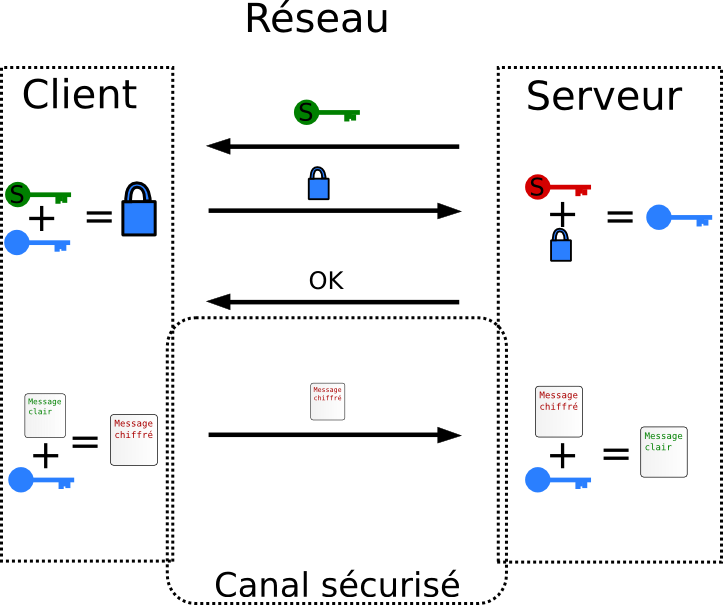
\includegraphics[width=0.85\textwidth]{images/SSH.png}
    \caption{La mise en place d'un canal sécurisé via SSH}
%    \vspace{-15pt}
\end{figure}

Ensuite, l'authentification se fait la plupart du temps via un
simple nom d'utilisateur et mot de passe, mais peut se faire via
l'utilisation des clés publiques : le serveur chiffre un message 
avec la clé
publique du client, et si celui ci parvient à le déchiffrer, il
sera identifié.
